\documentclass{article}

\usepackage{listings}
\usepackage{color}
\usepackage{graphicx}
\usepackage{float}
\usepackage{amsmath}
\usepackage{subfig}
\usepackage{cite}
\usepackage{url}
\usepackage{amsmath}

\newcounter{qcounter}

\begin{document}

\title{Image Analysis - TP5 - Lucas Kanade Tracker}

\author{Jander Nascimento, 
\and Raquel Oliveira}

\maketitle

\section{Introduction}

	Lucas Kanade is an algorithm that looks for the optimal parameters $\Delta_i$ and $\Delta_j$ that minimize the following equation:

	\begin{figure}[H]
		  \centering
		  \subfloat{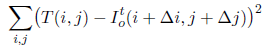
\includegraphics[width=0.4\textwidth]{img/form1.png}}
		  \caption{}
		  \label{fig:formula1}
	\end{figure}

	This equation can be solved using a classical mean squared method, which results in the following equation:

	\begin{figure}[H]
		  \centering
		  \subfloat{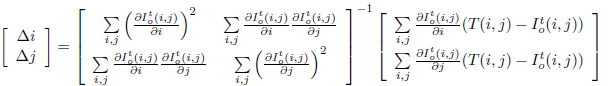
\includegraphics[width=1.0\textwidth]{img/form2.png}}
		  \caption{}
		  \label{fig:formula2}
	\end{figure}	

	In this practical work, we implemented the Lucas Kanade algorithm in order to track as object in a series of 139 images. First we implemented the interpolation function, then we implemented the algorithm itself to calculate $\Delta_i$ and $\Delta_j$, and finally we applied the algorithm in a series of images where an object is moving, and we placed a bound-box around the object in each image. The results will be explained in the following sections.


\section{Interpolation}

	Bilinear Interpolation is a method to generate a new image (given a initial image {\it I}) where the value of the pixels is a sum of the intensities of its four neighbors, weighted by the distance to the neighbor's center.

	For each pixel {\it(i,j)} of the original image {\it I}, the new pixel in the interpolated image {\it $I_w$} is calculated in the following manner:

	\begin{equation}
		I_w(i+\Delta_i^e , j+\Delta_j^e) += (1-\Delta_i^f)(1-\Delta_j^f)I(i,j)
	\end{equation}
	\begin{equation}
		I_w(i+\Delta_i^e+1 , j+\Delta_j^e) += \Delta_i^f(1-\Delta_j^f)I(i,j)
	\end{equation}
	\begin{equation}
  		I_w(i+\Delta_i^e , j+\Delta_j^e+1) += (1-\Delta_i^f)\Delta_j^fI(i,j)
	\end{equation}
	\begin{equation}
		I_w(i+\Delta_i^e+1 , j+\Delta_j^e+1) += \Delta_i^f \Delta_j^fI(i,j)
	\end{equation}

	where: 
		\begin{itemize}
			\item {\it $\Delta_i$} is the translation along {\it i}
			\item {\it $\Delta_j$} is the translation along {\it j} 
			\item {\it $\Delta^e$} is the integer part of the translation (ie: $\Delta=-5.3$, then ${\it \Delta^e}=-5$
			\item {\it $\Delta^f$} is the decimal part of the translation (ie: $\Delta=-5.3$, then ${\it \Delta^f}=0.3$
		\end{itemize}

	In the Figure \ref{fig:interp} we can see the result of an interpolation. It is possible to observe that the interpolated image, compared with the original image, is a little deformed, due to the fact that the pixels in the new image are interpolated with their neighbors.


	\begin{figure}[H]
		  \centering
		  \subfloat[Original image]{
\includegraphics[width=0.4\textwidth]{img/taz.png}}
		  \hspace{0.1cm}
		  \subfloat[Interpolated image ($\Delta_i=12.8   \Delta_j=-6.3$)]{
\includegraphics[width=0.4\textwidth]{img/taz0interp.png}}
		  \caption{Interpolation of an image}
		  \hspace{0.1cm}
		  \label{fig:interp}
	\end{figure}		

	

	After apply a translation ($\Delta_i,\Delta_j$) in an image, if we apply the inverse of the translation ($-\Delta_i,-\Delta_j$) on the same interpolated image we will not get the exactly the original image. This behavior can be seen in the Figure \ref{fig:inverseinterp}. Although the pixels return to their original position in the image, their intensities are not properly recovered. Another point to observe is that, when parts of the image are cut by the interpolation (for instance, the foot of Taz), they are not recovered either, due to the fact that they are not in the interpolated image anymore.

	\begin{figure}[H]
		  \centering
		  \subfloat[Original image]{
\includegraphics[width=0.3\textwidth]{img/taz.png}}
		  \hspace{0.1cm}
		  \subfloat[Interpolated image ($\Delta_i=12.8   \Delta_j=-6.3$)]{
\includegraphics[width=0.3\textwidth]{img/taz0interp.png}}
		  \hspace{0.1cm}
		  \subfloat[Inverse of the interpolation]{
\includegraphics[width=0.3\textwidth]{img/taz0interp_inverse.png}}
		  \caption{Inverse of the Interpolation}
		  \label{fig:inverseinterp}
	\end{figure}	



\section{Tracking an object}

	Here it is a case of Lucas Kanade application. We start from a template and an initial image (in Figure \ref{fig:template}). We calculate the error between the template and a part of the original image several times. At each time, using the equation described in Figure \ref{fig:formula2}, we calculate $\delta_i$ and $\delta_j$, in order to interpolate the image. We loop again until $\delta_i$ and $\delta_j$ reach a given threshold, when we stop the iterations and at this time we have the values of $\Delta_i$ and $\Delta_j$. 

\begin{figure}[H]
	  \centering
	  \subfloat[Template]{
\includegraphics[width=0.4\textwidth]{../image/report/taz.png}}
		  \hspace{0.1cm}
	  \subfloat[First Image]{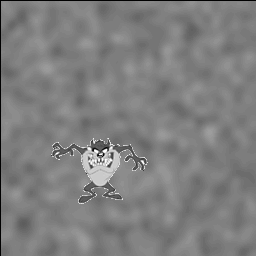
\includegraphics[width=0.4\textwidth]{img/taz001.png}}
	  \caption{Initial images}
	  \label{fig:template}
\end{figure}

	We applied the algorithm for a series of 139 images when an object is moving. As as example, we will illustrate that in the report with 3 images (Figure \ref{fig:sample}).


\begin{figure}[H]
\centering
\subfloat{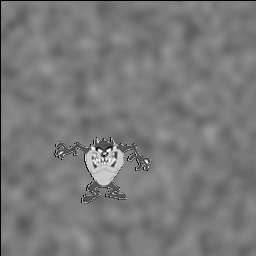
\includegraphics[width=0.3\textwidth]{../image/report/taz004_nb.png}}
		  \hspace{0.1cm}
\subfloat{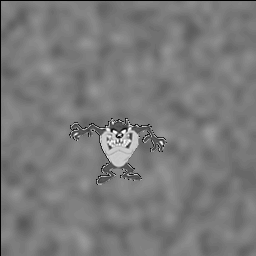
\includegraphics[width=0.3\textwidth]{../image/report/taz020_nb.png}}
		  \hspace{0.1cm}
\subfloat{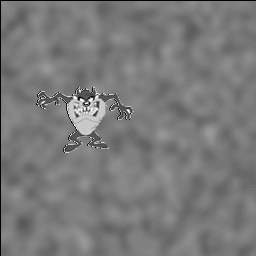
\includegraphics[width=0.3\textwidth]{../image/report/taz063_nb.png}}
\caption{Sample Images}
\label{fig:sample}
\end{figure}	

	In the first iteration, when we crop a part of the original image and compare with the template in order to find the first $\Delta_i$ and $\Delta_j$ ones, we already place a bounding box in the image. We repeat the process for all the images of the series, at each time step we find the new displacements $\Delta_i$ and $\Delta_j$ and we paint a bounding box around the tracked object (Figure \ref{fig:tracked}). 

	This algorithm enables the tracking of an object in the image sequence.

\begin{figure}[H]
\centering
\subfloat{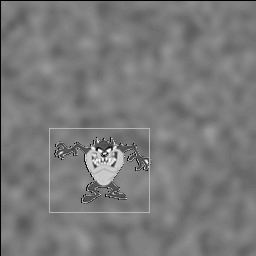
\includegraphics[width=0.3\textwidth]{../image/report/taz004_bb.png}}
		  \hspace{0.1cm}
\subfloat{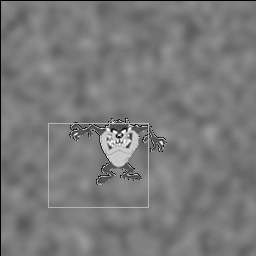
\includegraphics[width=0.3\textwidth]{../image/report/taz020_bb.png}}
		  \hspace{0.1cm}
\subfloat{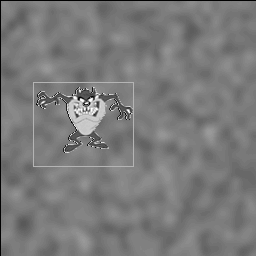
\includegraphics[width=0.3\textwidth]{../image/report/taz063_bb.png}}
\caption{Tracked Images}
\label{fig:tracked}
\end{figure}	


\section{Drawbacks}

Lucas Kanade has shown to be very efficient in some cases, now let's take a look in the situation where this algorithm does not work that well.

In large motions (at a higher speed) the tracker is not able to detect the changing region of the image with the correct direction vector.

And also if the image changes drastically its illumination, this can produce a wrong image evaluation.


\section{How to run?}

	Steps to compile the application:
	
	\begin{itemize}
		\item svn checkout https://jfimageanalysis.googlecode.com/svn/trunk/TP5/ \#download source code
		\item make \#compiles the code
	\end{itemize}

	As an input image only a set of {\bf pgm plaintext/ansii} files (P2), that should be stored in the directory \emph{images/tazplain/}. 

	Examples of usage:

	\begin{itemize}
		\item ./tp5
	\end{itemize}

	The resulting images will be generated in \emph{SRC/image/tazplain/result}.

\end{document}


